Please note that every single part of the following hardware
configuration is optional in the example applications. You do not need
any of the hardware present to develop with ARLib! This is the hardware we were
developing for:
\begin{itemize}
	\item{2x \href{http://www.logitech.com/de-de/product/hd-webcam-c310}{Logitech C310 Webcams}}
	\item{\href{https://github.com/ands/OculusMeetsAR/tree/master/Hardware/Printmodels}{3D-Printed camera mounts and lens mounts}}
	\item{2x \href{http://www.camera2000.com/en/cctv-board-security-video-camera-1-8mm-lens-f2-0.html}{Fisheye 1.8mm lens F2.0}}
	\item{\href{https://www.oculus.com/dk2/}{Oculus Rift DK2 Head-Mounted Display}}
	\item{\href{http://www.optitrack.com/products/flex-3/}{OptiTrack Flex 3 Tracking System}}
\end{itemize}

\begin{figure}[htb!]
	\centering
	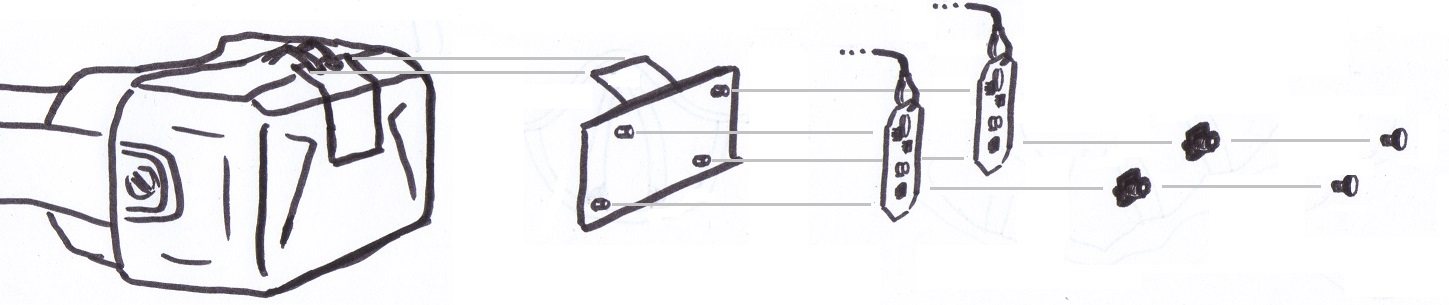
\includegraphics{explosion}
	\vspace{1mm}
	\caption{Exploded-view drawing of our modified HMD. The components from left to right: Oculus Rift DK2, 3D-printed camera mount, Logitech C310s, 3D-printed lens mounts, lenses.}
	\label{fig:explosion}
\end{figure}

\subsection{Lens selection and camera calibration}\label{lens-selection-and-camera-calibration}

Regarding our hardware choices we recommend William Steptoe's
\href{http://willsteptoe.com/post/67399683294/ar-rift-camera-selection-part-2}{documentation
on his project AR-Rift}. According to different user-reports, the actual
horizontal FOV of the DK2, which should be matched by the lenses, is
only about 80\textdegree-90\textdegree. With our lenses, we got a vertical* FOV of
approximately 75\textdegree, so for a more accurate matching one might want to buy
lenses with a smaller focal length. To prevent easy mistakes on your
search for other lenses, we recommend
\href{http://pomeroyprinting.blogspot.de/2014/04/modifying-logitech-c310-hd-webcam.html}{this
post by Brandon Pomeroy}.

For calibration we used Davide Scaramuzzas
\href{https://sites.google.com/site/scarabotix/ocamcalib-toolbox}{OCamCalib toolbox} along with a small
\href{https://github.com/ands/OculusMeetsAR/tree/master/Hardware}{stereo calibration tool}, we implemented using OpenCV. Click
\href{https://github.com/ands/OculusMeetsAR/wiki/Calibration}{here} for a step-by-step guide and technical details.
\\
\\
*Remark: This is the relevant FOV since the cameras are mounted with a 90\textdegree rotation!